Plan:
\textbf{Two Examples + Algorithm Overview}
\begin{itemize}
\item {Multiple-Path While Loop}
\\
\textbf{The First Challenge/Problem from The Example, 
and the Overview of the New Techniques Targeting This Problem}
\item {Nested While Loop}
\\
\textbf{The Second Challenge/Problem from The Example,
and the Overview of the New Techniques Targeting This Problem}
\end{itemize}
In this section, we discuss two representative examples with
challenges of analyzing the symbolic bounds for the reachability-bound.
We also give the technique overview for the analysis algorithm.
%
\subsection{Multiple-Path Loop}
\label{sec:overview-multiplepath}
\begin{example}
  [While Loop Example with Two Paths Iterating Alternatively]
  \label{ex:whileOdd}
  { \small
  \begin{figure}
  \centering
  \begin{subfigure}{.4\textwidth}
    \begin{centering}
    {\small
    $
    \begin{array}{l}
      \kw{whileOdd}(k) \triangleq \\
      \clabel{ \assign{i}{k} }^{0} ; \\
          \ewhile ~ \clabel{i > 0}^{1} ~ \edo ~ \\
          \qquad \Big(
            \eif(\clabel{i \% 2 = 0 }^{2},
            % \qquad \qquad 
            \clabel{\assign{i}{i - 1}}^{3},
            % \qquad \qquad 
            \clabel{\assign{i}{i - 3}}^{4});
            \Big)
      \end{array}
    $
    }
    \caption{}
    \end{centering}
    \end{subfigure}
  \begin{subfigure}{.5\textwidth}
    \begin{centering}
  %   \todo{abstract-cfg for two round}
  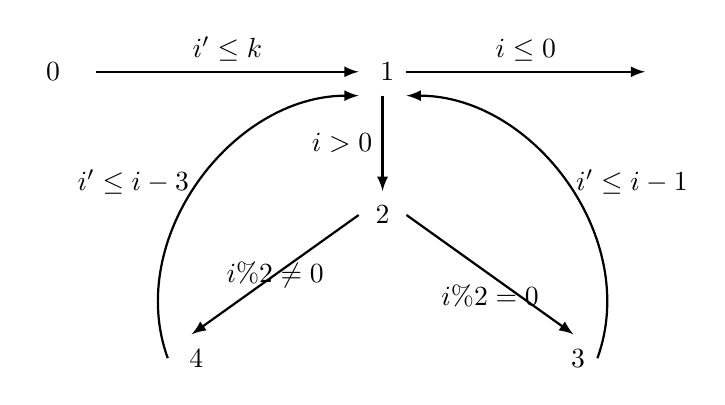
\begin{tikzpicture}[scale=\textwidth/20cm,samples=200]
  \draw[] (-7, 10) circle (0pt) node{{ $0$}};
  \draw[] (0, 10) circle (0pt) node{{ $1$}};
  \draw[] (0, 7) circle (0pt) node{\textbf{$2$}};
  \draw[] (4, 4) circle (0pt) node{{ $3$}};
  % \draw[] (0, 1) circle (0pt) node{{ $4$}};
  \draw[] (-4, 4) circle (0pt) node{{ $4$}};
  % Counter Variables
  \draw[] (6, 10) circle (0pt) node {\textbf{$\lex$}};
  % \draw[] (6, 4) circle (0pt) node {{ $ex$}};
  %
  % Control Flow Edges:
  \draw[ thick, -latex] (-6, 10)  -- node [above] {$i' \leq k$}(-0.5, 10);
  \draw[ thick, -latex] (0, 9.5)  -- node [left] {$i > 0$} (0, 7.5) ;
  \draw[ thick, -latex] (0.5, 7)  -- node [below] {$ i \% 2 = 0 $}  (4, 4.5);
  \draw[ thick, -latex] (-4.5, 4)  to  [out=110,in=180]  node [left] {$i' \leq i - 3$ }(-0.5, 9.5);
  \draw[ thick, -latex] (4.5, 4)  to  [out=70,in=0]   node [right] {$i' \leq i - 1$ }(0.5, 9.5);
  \draw[ thick, -latex]  (-0.5, 7) -- node  {$i \% 2 \neq 0$}  (-4, 4.5) ;
  \draw[ thick, -latex] (0.5, 10)  -- node [above] {$i \leq 0$}  (5.5, 10);
  % \draw[ thick, -latex] (6, 6.5)  -- node [right] {$\top$} (6, 4.5) ;
  \end{tikzpicture}
  \caption{}
    \end{centering}
    \end{subfigure}
  \caption{
  (a) The Simple While Loop Example with Two Paths Iterating Alternatively
    (b) The Abstract Execution Control Flow Graph}
      \label{fig:whileOdd}
  \end{figure}
  }
  %
  \end{example}    
  \begin{enumerate}
    \item  \textbf{The Abstract Execution Control Flow Graph} is generated in Figure~\ref{fig:whileOdd}(b).
    \item \textbf{Program Refinement}
    \\
    The loop free simple transition paths are computed as follows,
    \[
    \begin{array}{ll}
      \tpath_0 = (0 \to 1)
      &
      \tpath_1 = (1 \to 2), (2 \to 3), (3 \to 1)
      \\
      \tpath_2 = (1 \to 2), (2 \to 4), (4 \to 1)
      &
      \tpath_3 = (1 \to \lex)
    \end{array}
    \]
  \textbf{Refined Program}:
  \[
    \tpath_0 ; \rpchoose{1: \rprepeat(\tpath_1; \tpath_2) , 
    1: \rprepeat(\tpath_2; \tpath_1)}; \tpath_3
    \]
  \item \textbf{Outside-In Algorithm} : Compute Local Bound for Every program and sub programs.
  \[
    \begin{array}{lll}
      \outinB(\tpath_0) = 1
      &
      \outinB(\tpath_3) = 1
      &
      \outinB(\rprepeat(\tpath_1; \tpath_2)) = \frac{n}{4} 
      \\
      \outinB(\tpath_1) = 1 
      &
      \outinB(\tpath_2) = 1 
      &
      \outinB(\rprepeat(\tpath_2; \tpath_1)) = \frac{n}{4}
    \end{array}
    \]
  %       $\outinB(\tpath_0) = 1$
  % \\
  % $\outinB(\tpath_3) = 1$
  % \\
  % $\outinB(\tpath_1) = 1 $
  % \\
  % $\outinB(\rprepeat(\tpath_1; \tpath_2)) = \frac{n}{4} $
  % \\
  % $\outinB(\tpath_2) = 1 $
  % \\
  % $\outinB(\rprepeat(\tpath_2; \tpath_1)) = \frac{n}{4} $
  % \\
  % $\outinB(1: \rpchoose(\rprepeat_2(\cdots), \tpath_1)) 
  % = \max\{m, \frac{n}{m}\} $
  % \\
  \item \textbf{Inside-Out Algorithm}
  \begin{itemize}
    \item \textbf{Repeat Chain Set}
    \\
    $\rpchset(1, \tpath_1) = \{ \rprepeat(\tpath_1; \tpath_2) \to \tpath_1\}$ \\
    $\rpchset(1, \tpath_2) = \{ \rprepeat(\tpath_2; \tpath_1) \to \tpath_2\}$ \\
    $\rpchset(\_, \_) = \emptyset$ 
    % \\
    \item \textbf{Repeat Chain Bound} for every simple transition path $\tpath$ through its \emph{Repeat Chain}s
    $\rpchB(1, \tpath_1) = \frac{n}{4}$ \\
    $\rpchB(1, \tpath_2) = \frac{n}{4}$ 
    %
    \item \textbf{Loop Chain}
    \[
      % \begin{array}{ll}
        \lpch(\tpath_1) = 1 \to \tpath_1
        \quad
        \lpch(\tpath_2) = 1 \to \tpath_2
        \quad
        \lpch(\tpath_0) = \tpath_0
        \quad
        \lpch(\tpath_3) = \tpath_3
      % \end{array}
      \]
    % $\lpch(\tpath_1) = \{1\to \tpath_1\}$ \\
    % $\lpch(\tpath_2) = \{1\to \tpath_2\}$ \\
    % $\lpch(\tpath_0) = \{\tpath_0\}$ \\
    % $\lpch(\tpath_3) = \{\tpath_3\}$ 
    \item \textbf{{Relative Loop Bound}} for every simple transition path $\tpath$ through its \emph{Loop Chain}
    \[
    %   \begin{array}{ll}
        \rpchB(1, \tpath_1) = \frac{n}{4}
        \qquad
        \rpchB(1, \tpath_2) = \frac{n}{4}
        \qquad
        \rpchB(\bot, \tpath_0) = 1
        \qquad
        \rpchB(\bot, \tpath_3) = 1
      % \end{array}
      \]
    % $\rpchB(1, \tpath_1) = \frac{n}{4}$ \\
    % $\rpchB(1, \tpath_2) = \frac{n}{4}$  \\
    % $\rpchB(\bot, \tpath_0) = 1$ \\
    % $\rpchB(\bot, \tpath_3) = 1$ 
    \item \textbf{Path-Sensitive Reachability-Bound} for every simple transition path $\tpath$
    \\
    $\inoutB(\tpath_1) = \frac{n}{4}$ \quad
    $\inoutB(\tpath_2) = \frac{n}{4}$ \quad
    $\inoutB(\tpath_0) = 1$ \quad
    $\inoutB(\tpath_3) = 1$ 
  \end{itemize}
  \item \textbf{Path Sensitive Reachability-Bound} on every program control location
  \\
  $\psRB(\{0, \lex\}) = 1$ \quad
  $\psRB(\{3, 4 \}) = \lfloor \frac{n}{4} \rfloor$ \quad
  $\psRB(\{2, 1\}) = \lfloor \frac{n}{2} \rfloor + 1$ \quad
  \end{enumerate}
Figure~\ref{fig:whileOdd}(a) shows an example of the multiple path loops
with different iterations for different paths.
This example is simplified from the example in~\cite{Sumit2010rechability}, which
is a skeleton code from the .Net base-class library.
\\
In this example,
the precise reachability-bounds for control location $3$ and $4$ are both $\frac{k}{4}$,
$\frac{k}{2}$ for location $2$, and $\frac{k}{2} + 1$ for location $1$.
\\
In order to know location $3$ and $4$ are executed $\frac{k}{4}$,
we need to know location $3$ and $4$ is executed alternatively after each other.
In other words, neither of them is executed twice in 2 consecutive iterations.
\\
However, by paper~\cite{Sumit2010rechability} where the \emph{reachability-bound} problem is defined,
it can only derive the bound $k$ for location $3$ and $4$ by their path-insensitive method.
To best of my knowledge, there isn't any other later works solving the \emph{reachability-bound} problem.
\\
Among the works on loop bound analysis, \cite{GulwaniJK09} can compute the precise global
loop bound (i.e., $\frac{k}{2}$) for this simple example in a path-sensitive way.
Using this global bound, we can compute the reachability-bound for location $1$ and $2$.
However, reachability-bound for control location $3$ and $4$ are still unclear.
% In order to know location $3$ and $4$ are executed $\frac{k}{4}$,
% we need to know location $3$ and $4$ is executed alternatively after each other.
% In other words, neither of them is executed twice in 2 consecutive iterations.
% \\
% We need to generate the repeat patterns containing the two execution paths reflecting this property.
% % However, this execution path corresponds to two iterations of the while loop.
% \\
% Then, we recover the \emph{reachability-bound} of location $3$ and $4$ globally from the
% repeat pattern through the \emph{Inside-Out} Algorithm introduced next.
% we need to 
\paragraph*{Outside-In Algorithm}
The first key idea of this path-sensitive \emph{reachability-bound} algorithm is the \emph{outside-in} algorithm.
\\
This algorithm combines the idea of DC-based program abstraction from \cite{sinn2017complexity}
and the while loop refinement~\cite{GulwaniJK09} efficient.
It first generates the constraint program based on the Difference constraint and refines every while loop in this constraint program.
Each refined while loop in the program is composed of its all possible repeat patterns.
Then it
computes the bound for every possible repeat pattern of the execution paths for every while loop,
in the direction
from its outermost repeat pattern to its innermost repeat pattern.
\\
% and the while loop refinement~\cite{GulwaniJK09}.
For this $\kw{whileOdd}$ example, the \emph{Outside-In} algorithm generates 
the repeat patterns containing the two execution paths reflecting this property.
There are 4 possible repeat patterns for this example:
\\
$\rprepeat(2 \to 3 \to 1; 2 \to 4 \to 1)$.
\\
$\rprepeat(2 \to 3 \to 1; 2 \to 4 \to 1)$.
\\
$2 \to 3 \to 1$
\\
$2 \to 4 \to 1$.
\\
\emph{Outside-In} computes the bound for every repeat pattern
as $\frace{k}{4}$, $\frac{k}{4}$, $1$, and $1$ respectively.
\\
Then in the next step, we recover the \emph{reachability-bound} of location $3$ and $4$ globally from the
repeat pattern through the \emph{Inside-Out} Algorithm.
\subsection{Nested Loops with Related Iterator}
\label{sec:overview-nestedwhile}
Figure~\ref{fig:threeWhile}(a) shows an example of the nested loops with related 
iterators.
This example is adopted from the example in~\cite{GulwaniJK09}, which is common in product code.
\\
In line 8, $i$ is reset by $w$ and $w$ is reset by $j$ at line 5. So we know the
while $LOOP_6$ is only executed in the first iteration of while loop 1 and 3.
\\
We also know while loop $LOOP_3$ at line 3 is executed only in 
the first $m - N$ iterations of the 
$LOOP_1$ because $j$ is reset by $i$ in line 2.
\\
So the total combined iterations of all the three loops is bounded above by 
$n + m^2 - m \times N$.
\\
So far, The loop bound analysis method in \cite{GulwaniJK09} is able to give
an approximation for the $n + (m \times n) + N$. 
The DC-based algorithm in \cite{sinn2017complexity} is able to
compute the precise combined loop bound of $n + m^2 - m \times N$.
\\
However, knowing the global loop bound isn't enough to solve the \emph{reachability-bound problem} for locations inside
$LOOP_6$.
\\
% However, i
% In order to solve the \emph{reachability-bound problem} for locations inside
In order to how many times the locations inside
$LOOP_6$ is executed globally, we need to know
how many iterations of the $LOOP_3$ and $LOOP_1$, 
during which the $LOOP_6$ is executed.
Then multiply the local bound of $LOOP_6$ with the iterations during which it can be touched.
\\
The Progress Invariant method in \cite{GulwaniJK09} is only able to compute
the loop bound for $LOOP_6$ inside $LOOP_3$ and $LOOP_1$.
So we have to over-approximate the global bound for $LOOP_6$ with the
overall program complexity, i.e., $n + m^2 - m \times N$.
\\
For the same reason, the DC-based algorithm in \cite{sinn2017complexity}
is only able to
compute the precise combined loop bound and the local bound of each loop
separately as well.
We are still unable to know the  \emph{reachability-bound} for the locations in the innermost loop.
% \\
\paragraph*{Inside-Out Algorithm}
The second key idea of this path-sensitive reachability analysis algorithm is the
\emph{inside-out} algorithm.
This algorithm computes an \emph{Inside-Out} bound on number of the iterations for
every nested outside loop w.r.t. the innermost loop of every control location.
Such that during these iterations, the innermost loop is touched. 
% the for every program control location,
% how many times the innermost loop of this control location will be touched w.r.t. every
% outside loop it is nested in.
This is distinguished from the traditional methods, which compute the local bound
of the innermost loop w.r.t. the outside loop it is nested in.
%
\\
For this nested loop program $\kw{threeNestedWhile}$, 
we compute the \emph{Inside-Out} bound for $LOOP_1$ and $LOOP_3$
w.r.t. the $LOOP_6$ as follows,
$InOut(LOOP_1, LOOP_6) = 1$.
\\
$InOut(LOOP_3, LOOP_6) = 1$.
Then, we combine this result with the local bound
computed from the \emph{Outside-In} algorithm.
For the only one path $6 \to 7$ in $LOOP_6$, 
we compute the accurate reachability bound $N$.
\\
Finally, the derivation of the reachability bound for location $6$ and $7$
on this path is straightforward.
\begin{example}[Nested Loop with Related Iterators]
  \label{ex:threeNestedWhile}
  %
  %
  { \small
\begin{figure}
\centering
\begin{subfigure}{.4\textwidth}
  \begin{centering}
  {\footnotesize
  $
  \begin{array}{l}
      \kw{relatedNestedWhile}(n, m, N) \triangleq \\
      \clabel{ \assign{i}{0} }^{0} ; \\
          \ewhile ~ \clabel{i < n}^{1} ~ \edo ~ \\
          \qquad \Big(
           \clabel{\assign{j}{m}}^{2} ;\\
           \qquad \ewhile ~ \clabel{j > 0}^{3} ~ \edo ~ \\
           \qquad \qquad \Big(
            \clabel{\assign{j}{j-1}}^{4};
            \clabel{\assign{w}{i}}^{5};\\
            \qquad \qquad \ewhile ~ \clabel{w < N}^{6} ~ \edo ~
            \Big(
              \clabel{\assign{w}{w + 1}}^{7}
                \Big); \\
                \qquad \qquad \clabel{\assign{i}{w}}^{8}
                \Big); \\
                \qquad \clabel{\assign{i}{i+1}}^{9}
            \Big)
      \end{array}
  $
  }
  \caption{}
  \end{centering}
  \end{subfigure}
\begin{subfigure}{.5\textwidth}
  \begin{centering}
%   \todo{abstract-cfg for two round}
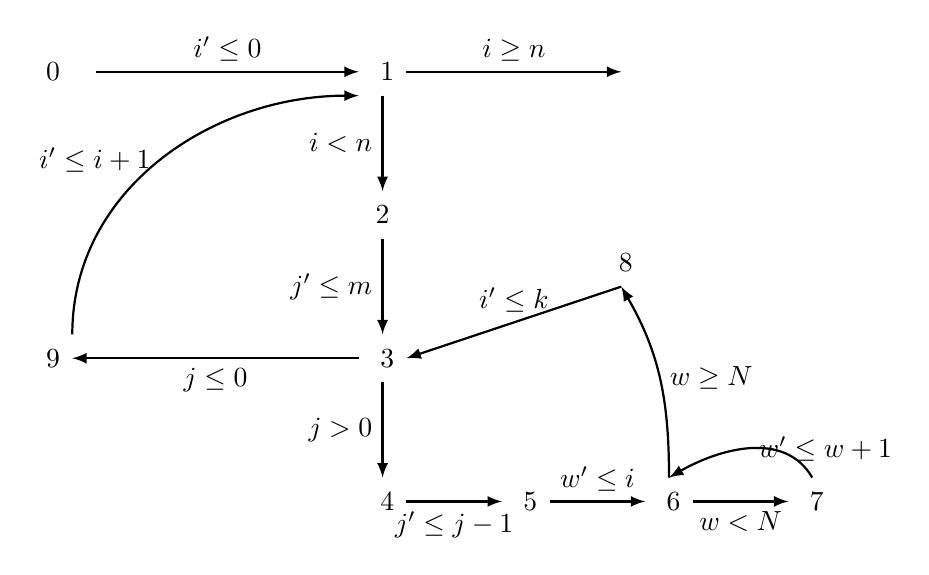
\begin{tikzpicture}[scale=\textwidth/20cm,samples=200]
\draw[] (-7, 10) circle (0pt) node{{ $0$}};
\draw[] (0, 10) circle (0pt) node{{ $1$}};
\draw[] (6, 10) circle (0pt) node {{$\lex$}};
\draw[] (0, 7) circle (0pt) node{{$2$}};
\draw[] (0, 4) circle (0pt) node{{ $3$}};
\draw[] (-7, 4) circle (0pt) node{{ $9$}};
\draw[] (0, 1) circle (0pt) node{{ $4$}};
\draw[] (3, 1) circle (0pt) node{{ $5$}};
\draw[] (6, 1) circle (0pt) node{{ $6$}};
\draw[] (9, 1) circle (0pt) node{{ $7$}};
\draw[] (5, 6) circle (0pt) node{{ $8$}};
% Counter Variables
%
% Control Flow Edges:
\draw[ thick, -latex] (-6, 10)  -- node [above] {$i' \leq 0$}(-0.5, 10);
\draw[ thick, -latex] (0, 9.5)  -- node [left] {$i < n$} (0, 7.5) ;
\draw[ thick, -latex] (0, 6.5)  -- node [left] {$j' \leq m$} (0, 4.5) ;
\draw[ thick, -latex] (0, 3.5)  -- node [left] {$j > 0$} (0, 1.5) ;
\draw[ thick, -latex] (-0.5, 4)  -- node [below] {$j \leq 0$} (-6.5, 4) ;
\draw[ thick, -latex] (-6.5, 4.5)  to  [out=90,in=180]  node [left] {$i' \leq i + 1$ }(-0.5, 9.5);
\draw[ thick, -latex] (0.5, 10)  -- node [above] {$i \geq n$}  (5, 10);
\draw[ thick, -latex] (0.5, 1)  -- node [below] {$j' \leq j - 1$}  (2.5, 1);
\draw[ thick, -latex] (3.5, 1)  -- node [above] {$w' \leq i$}  (5.5, 1);
\draw[ thick, -latex] (6.5, 1)  -- node [below] {$w < N$}  (8.5, 1);
\draw[ thick, -latex] (6, 1.5)  to [out=90,in=-60] node [right] {$w \geq N$}  (5, 5.5);
\draw[ thick, -latex] (9, 1.5)  to  [out=120,in=30] node [right] {$w' \leq w + 1$}  (6, 1.5);
\draw[ thick, -latex] (5, 5.5)  to  node [above] {$i' \leq k$ }(0.5, 4);
\end{tikzpicture}
\caption{}
  \end{centering}
  \end{subfigure}
\caption{
(a) The Example of Nested Loop with Related Iterators
  (b) The Abstract Execution Control Flow Graph}
    \label{fig:threeNestedWhile}
\end{figure}
}
\end{example}

\begin{enumerate}
  \item  \textbf{The Constraint Program (Abstract Control Flow Graph)} is generated in Figure~\ref{fig:threeNestedWhile}(b).

  \item \textbf{Program Refinement}
  \\
  The loop free simple transition paths are computed as follows,
  \[
      \begin{array}{llll}
          \tpath_0 = (0 \to 1)
          &
          \tpath_1 = (1 \to 2), (2 \to 3)
          &           
          \tpath_2 = (3 \to 4), (4 \to 5), (5 \to 6)
          &
          \tpath_3 = (6 \to 7), (7 \to 6)
          \\
          \tpath_6 = (1 \to \lex)
          &
          \tpath_4 = (6 \to 8), (8 \to 3)
          &
          \tpath_5 = (3 \to 9), (9 \to 1)
      \end{array}
      \]
  \textbf{Refined Program}:
  \[
  \rprog = \tpath_0 ; 1: \rprepeat(\tpath_1; 3: \rprepeat(\tpath_2; 6 : \rprepeat(\tpath_3); \tpath_4); \tpath_5); \tpath_6
  \]
  \item \textbf{Outside-In Algorithm} :The \emph{OutIn} bound for the $\rprog$ and every nested repeat patterns.
  \\
$\outinB(\tpath_0) = 1$
\quad
$\outinB(\tpath_6) = 1$
\quad
$\outinB(6 : \rprepeat(\tpath_3)) = N $
\\
$\outinB(3: \rprepeat(\tpath_2; 6 : \rprepeat(\tpath_3); \tpath_4)) = m $
\\
$\outinB(1: \rprepeat(\tpath_1; 3: \rprepeat(\tpath_2; 6 : \rprepeat(\tpath_3); \tpath_4); \tpath_5)) = n - N $
\item \textbf{Inside-Out Algorithm}
\begin{itemize}
  \item \textbf{Repeat Chain Set}
  \\
  $\rpchset(1, \tpath_1) = \{1: \rprepeat(\tpath_1; 3: \rprepeat(\tpath_2; 6 : \rprepeat(\tpath_3); \tpath_4); \tpath_5)\}$
  \\
  $\rpchset(1, \tpath_5) = \{1: \rprepeat(\tpath_1; 3: \rprepeat(\tpath_2; 6 : \rprepeat(\tpath_3); \tpath_4); \tpath_5)\}$
  \\
  $\rpchset(3, \tpath_2) = \{3: \rprepeat(\tpath_2; 6 : \rprepeat(\tpath_3); \tpath_4)\}$
  \\
  $\rpchset(3, \tpath_4) = \{3: \rprepeat(\tpath_2; 6 : \rprepeat(\tpath_3); \tpath_4)\}$
  \\
  $\rpchset(6, \tpath_3) = \{6: \rprepeat(\tpath_3)\}$
  \\
  $\rpchset(_, \_) = \emptyset$ 
  % \\
  \item \textbf{Repeat Chain Bound} for every simple transition path $\tpath$ through its \emph{Repeat Chain}s
  \\
  $\rpchB(1, \tpath_1) = n - N$ \quad
  $\rpchB(1, \tpath_5) = n - N$ \quad
  $\rpchB(3, \tpath_2) = m$ \\
  $\rpchB(3, \tpath_4) = m$ \quad
  $\rpchB(6, \tpath_3) = N$ \quad \quad 
  $\rpchB(_, \_) = \bot $ 
  %
  \item \textbf{Loop Chain}
  \\
  $\lpch(\tpath_1) = 1\to \tpath_1$ \quad
  $\lpch(\tpath_2) = 1 \to 3 \to \tpath_2$ \\
  $\lpch(\tpath_5) = 1\to \tpath_5$ \quad
  $\lpch(\tpath_4) = 1 \to 3 \to \tpath_4$ \\
  \highlight
  {$\lpch(\tpath_3) = 1 \to 3 \to 5 \to \tpath_3$ }\\
  $\lpch(\tpath_0) = \tpath_0$ \quad
  $\lpch(\tpath_6) = \tpath_6$ 
  \item \textbf{{Relative Loop Bound}} for every simple transition path $\tpath$ through its \emph{Loop Chain}
  \\
  $\rpchB(1, \tpath_1) = n - N$ \\
  $\rpchB(1, \tpath_5) = n - N$ \\
  $\rpchB(1, \tpath_2) = n$; \quad $\rpchB(3, \tpath_2) = m$; \\
  $\rpchB(1, \tpath_4) = n$; \quad $\rpchB(3, \tpath_4) = m$ \\
  \highlight{$\rpchB(1, \tpath_3) = 1$; \quad $\rpchB(3, \tpath_3) = 1$; \quad $\rpchB(5, \tpath_3) = N$} \\
  $\rpchB(_, \_) = \bot $ 
  \item \textbf{Path-Sensitive Reachability-Bound} for every simple transition path $\tpath$
  \\
  $\inoutB(\tpath_1) = n - N$ \quad
  $\inoutB(\tpath_2) = n \times m$ \quad
  $\inoutB(\tpath_0) = 1$ 
  \\
  $\inoutB(\tpath_5) = n - N$ \quad
  $\inoutB(\tpath_4) = n \times m$ \quad
  $\inoutB(\tpath_6) = 1$ 
  \\
  $\inoutB(\tpath_3) = N$ \quad
\end{itemize}
\item \textbf{Path Sensitive Reachability-Bound} on every program control location
\\
$\psRB(\{0, \lex\}) = 1$ \quad
$\psRB(\{1\}) = n - N + 1$ \quad
$\psRB(\{2, 9\}) = n - N$ \quad
$\psRB(\{3\}) = n - N + n \times m$ \quad
$\psRB(\{4, 5, 8\}) = n \times m$ \quad
$\psRB(\{7\}) = N$ \quad
$\psRB(\{6\}) = N + n \times m$ 
\end{enumerate}
